\documentclass[letterpaper,11pt]{article}
\usepackage{graphicx}
\graphicspath{ {images/} }
\usepackage{wrapfig}
\usepackage{lipsum}
\newlength{\outerbordwidth}
\pagestyle{empty}
\raggedbottom
\raggedright
\usepackage[svgnames]{xcolor}
\usepackage{framed}
\usepackage{tocloft}
\usepackage{amsmath}
\usepackage{etoolbox}
\robustify\cftdotfill

%-----------------------------------------------------------
%Edit these values as you see fit
\setlength{\outerbordwidth}{3pt}  % Width of border outside of title bars
\definecolor{shadecolor}{gray}{0.75}  % Outer background color of title bars (0 = black, 1 = white)
\definecolor{shadecolorB}{gray}{0.93}  % Inner background color of title bars

%-----------------------------------------------------------
%Margin setup
\setlength{\evensidemargin}{-0.25in}
\setlength{\headheight}{-0.25in}
\setlength{\headsep}{0in}
\setlength{\oddsidemargin}{-0.25in}
\setlength{\paperheight}{11in}
\setlength{\paperwidth}{8.5in}
\setlength{\tabcolsep}{0in}
\setlength{\textheight}{9.75in}
\setlength{\textwidth}{7in}
\setlength{\topmargin}{-0.3in}
\setlength{\topskip}{0in}
\setlength{\voffset}{0.1in}

%-----------------------------------------------------------
%Custom commands
\newcommand{\resitem}[1]{\item #1 \vspace{-2pt}}
\newcommand{\resheading}[1]{\vspace{8pt}
  \parbox{\textwidth}{\setlength{\FrameSep}{\outerbordwidth}
    \begin{shaded}

\setlength{\fboxsep}{0pt}\framebox[\textwidth][l]{\setlength{\fboxsep}{4pt}\fcolorbox{shadecolorB}{shadecolorB}{\textbf{\sffamily{\mbox{~}\makebox[6.762in][l]{\large #1} \vphantom{p\^{E}}}}}}
    \end{shaded}
  }\vspace{-5pt}
}

\newcommand{\ressubheading}[4]{
\begin{tabular*}{6.5in}{l@{\cftdotfill{\cftsecdotsep}\extracolsep{\fill}}r}
		\textbf{#1} & #2 \\
		\textit{#3} & \textit{#4} \\
\end{tabular*}\vspace{-6pt}}
%--------------------------------------------------------------------------------------
\begin{document}

%---------------------Personal Information--------------------------------
%---------------------Image Inserted---------------------------------------
\begin{wrapfigure}{r}{4.5cm}
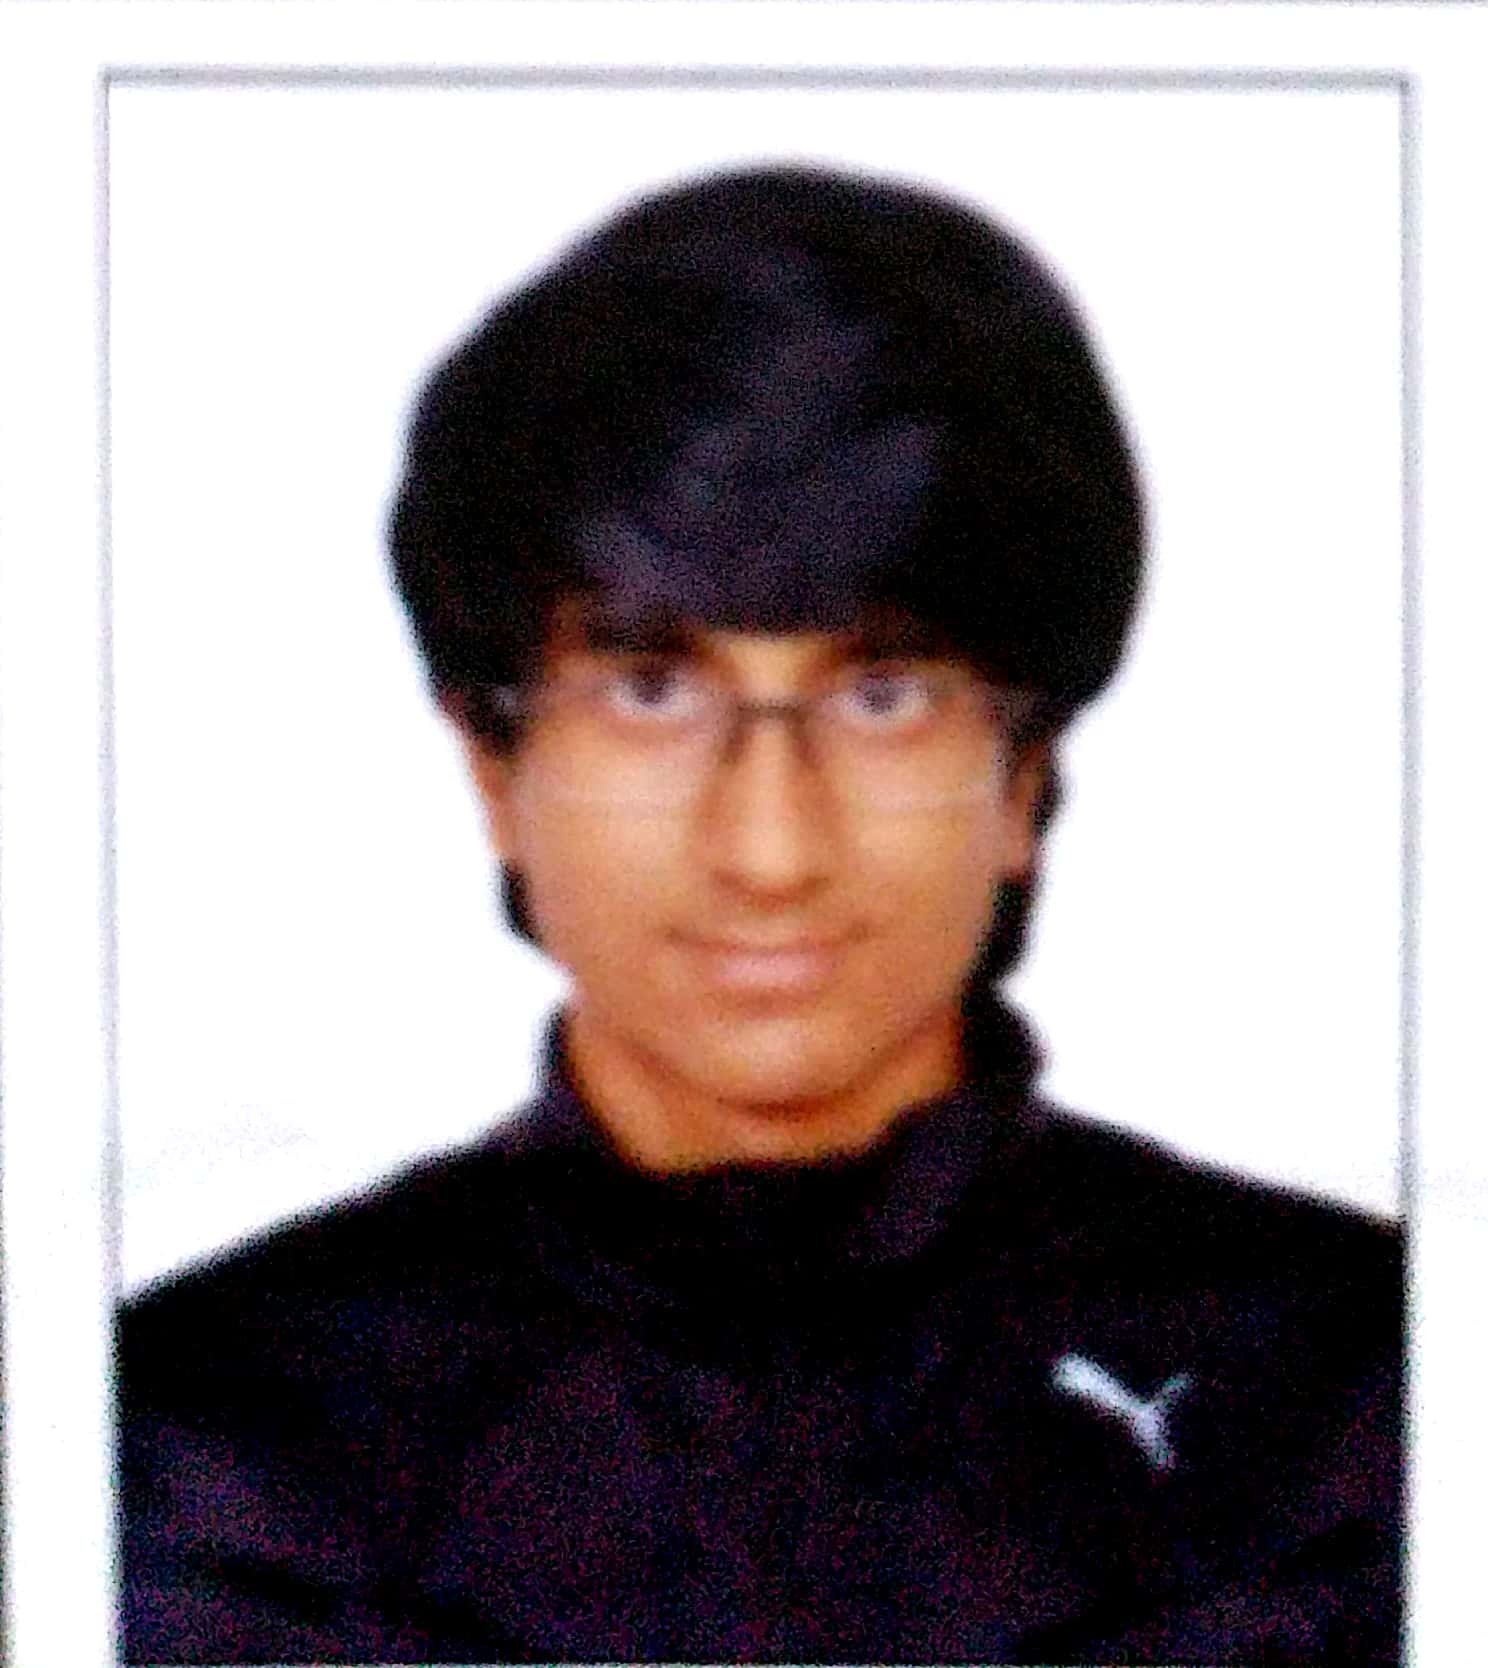
\includegraphics[width=2.5cm]{PHOTO}
\end{wrapfigure} 
%------------------------------------------
\textbf{}  \\
\textbf{{\Large Chirag Shah}}  \\
Email \hspace{0.2cm}  : chirag.ms@somaiya.edu \\
Contact : 9757084146 \\
Address : H-32, 1/2, Panchkamal C.H.S, Sector-29, \\
\hspace{1.8cm}Vashi, Navi Mumbai - 400703 \\ 
Linkedin : https://www.linkedin.com/in/chirag-shah-9b1a70b0
%\textbf{}  \\
%------------------------------------------------------------------------------

%----------------------------Career Objective-------------------------------
\resheading{Career Objective}
\textbf{}  \\
Self-Motivated engineering student, trying to develop innovative solutions to simplify tasks through robotics and information technology. Aiming to develop solutions, to improve the efficiency and qualtiy of manual tasks through assistive robotics \\

%-------------------Education--------------------------------------------------
\resheading{Education}

\begin{table}[h!]
  \begin{center}
      \begin{tabular}{l|c|r|l} % <-- Alignments: 1st column left, 2nd middle and 3rd right, with vertical lines in between
      \hspace{0.2cm}\textbf{Year}\hspace{0.2cm} &\hspace{0.2cm} \textbf{Degree/Certificate}\hspace{0.2cm} &\hspace{0.2cm} \textbf{Institute}\hspace{2.3cm} &\hspace{0.2cm} \textbf{CGPA / Percentage}\hspace{0.2cm}\\
      \hline
       2012 & \hspace{0.2cm} Secondary School Certificate \hspace{0.2cm} & \hspace{0.2cm}Fr. Agnel School\hspace{1.7cm} & \hspace{1.2cm} 95.09\% \hspace{0.2cm}\\
       2014 & \hspace{0.2cm} Higher Secondary School Certificate \hspace{0.2cm} & \hspace{0.2cm}Fr. Agnel School\hspace{1.7cm} & \hspace{1.2cm} 86.08\% \hspace{0.2cm}\\
      2014 & \hspace{0.2cm} 1st Semester Btech EXTC \hspace{0.2cm} & \hspace{0.2cm}K.J. Somaiya College of Engineering\hspace{0.2cm} & \hspace{1.2cm} 7.65 \hspace{0.2cm}\\
		2015 & \hspace{0.2cm} 2nd Semester Btech EXTC \hspace{0.2cm} & \hspace{0.2cm}K.J. Somaiya College of Engineering\hspace{0.2cm} & \hspace{1.2cm} 8.54 \hspace{0.2cm}\\
		2015 & \hspace{0.2cm} 3rd Semester Btech EXTC \hspace{0.2cm} & \hspace{0.2cm}K.J. Somaiya College of Engineering\hspace{0.2cm} & \hspace{1.2cm} 8.17 \hspace{0.2cm}\\
		2016 & \hspace{0.2cm} 4th Semester Btech EXTC \hspace{0.2cm} & \hspace{0.2cm}K.J. Somaiya College of Engineering\hspace{0.2cm} & \hspace{1.2cm} 8.8 \hspace{0.2cm}\\
		2016 & \hspace{0.2cm} 5th Semester Btech EXTC \hspace{0.2cm} & \hspace{0.2cm}K.J. Somaiya College of Engineering\hspace{0.2cm} & \hspace{1.2cm} 8.24 \hspace{0.2cm}\\
		2017 & \hspace{0.2cm} 6th Semester Btech EXTC \hspace{0.2cm} & \hspace{0.2cm}K.J. Somaiya College of Engineering\hspace{0.2cm} & \hspace{1.2cm} 8.32 \hspace{0.2cm}\\
		2017 & \hspace{0.2cm} 7th Semester Btech EXTC \hspace{0.2cm} & \hspace{0.2cm}K.J. Somaiya College of Engineering\hspace{0.2cm} & \hspace{1.2cm} 9.32 \hspace{0.2cm}\\
		      
          \end{tabular}
  \end{center}
\end{table}

EXTC - Electronics annd Telecommunication \\

%--------------------------Projects----------------------------------------------------------------
\resheading{Projects}
\textbf{}  \\
\textbf{Autonomous Water Rover} (July 2017 - Present): \\
An autonomous lake monitoring system is being developed, which can also be used for other applications such as depth mapping, fish finding etc. \\
\textbf{}  \\
\textbf{Robo-Rehab} (December 2017 - Present): \\
A continuous passive motion device for the arm, is being developed to aid physiotherapists in rehabilitation of paralysis victims.
\textbf{}  \\
\textbf{}  \\
\textbf{Anomaly Detection in a Bottling Plant} (December 2017 - March 2018): \\
A computer vision based system was designed to detect anomalies such as under filling, over filling in a bottling plant.
\textbf{}  \\
\textbf{}  \\
\textbf{SONAR using AVR and Matlab} (March 2016): \\
An ultrasound sensor mounted on a servo was used to get obstacles in a 180 degree field of vision and the results were plotted using matlab.
\textbf{}  \\
\textbf{}  \\
\textbf{Robocon} (November 2015 - March 2016)\\
\textbf{}  \\
\textbf{}  \\
\textbf{Robocon} (November 2016 - March 2017)\\
\textbf{}  \\
\textbf{Intrusion Detection System} (Jan 2015-July 2015): \\
A network IDS was developed using C\# ,as an intern in LucideusTech pvt. Ltd a company, incubated at SINE IIT B.
\textbf{}  \\
%--------------------------------------Internship and Trainings---------------------------------
\resheading{Internships and Trainings}
\textbf{}  \\
\textbf{1. Software Developer at Lucideus Tech Pvt.Ltd (Jan 2015-July 2015)} \\
A network Intrusion Detection System was developed using C\# and various cyber security related concepts were understood. 
\textbf{}  \\
\textbf{}  \\
\textbf{2. Co-Founder of Infigyaan (Oct 2016-Dec 2017)} \\
Co-founded a campus company turned partnership firm to provide android development training and internships to students in engineering colleges. The firm was dissolved in December 2017.
\textbf{}  \\
\textbf{}  \\
\textbf{3. Student at Eduvance Summer Industrial Training (May 19 2017- June 19 2017)} \\
In the Summer Industrial Training in Embedded Systems and IoT, at K.J. Somaiya College of Engineering concepts related to embedded systems, IoT were understood and implemented. ARM University and Cypress Semiconductors University Alliance certificates were also earned in the same course.
\textbf{}  \\
\textbf{}  \\
\textbf{4. Teaching Assistant at Eduvance (June 19 2017- July 13 2017)} \\
Assisted the conduction of Summer Industrial Training in Embedded Systems and IoT at SIES graduate School of Technology \\
\textbf{} 
\textbf{}  \\
\textbf{5. Teaching Assistant at Ekagrata NGO (March 19 2016- July 13 2017)} \\
Conducted a fifteen day, basic electronics workshop using kits provided by Eduprime pvt. Ltd for underpriviliged kids in Dharavi. 
\textbf{} \\
\textbf{}  \\
\textbf{6. Marine Robotics Worshop at National Institute of Oceanography (Feb 12 2018- Feb 17 2018)} \\
Attended a worshop on marine robotics which was taught by eminent professors and scientists from around the globe. 
\textbf{} 
%--------------------------------------Research Publications---------------------------------
\resheading{Research Publications}
\textbf{}  \\
\textbf{Bottling Line Inspection System using Digital Image Processing : } \\
Presented at 'ICIES 2018: 1st International Conference on Interdisciplinary Engineering and Sciences-2018 Pune, India, March 23-24, 2018' The paper will be published in the International Journal of Computer Applications (IJCA). 

%--------------------------------------Positions of Responsibilty---------------------------------
\resheading{Positions of Responsibilty}
\textbf{}  \\
\textbf{1. Captain of the Table Tennis Team of KJSCE (June 19 2015- March 19 2018)} \\
\begin{itemize}
  \item Won Silver at Mummbai Unversity, Men's Team Event in 2014 and 2015.   
  \item Won Gold at Skream, Men's Team Event in 2014 and 2016. 
\end{itemize}
\textbf{} 
\textbf{2. Sports Secretary (June 2016-May 2017)} \\
\begin{itemize}
  \item Head of the organising committee of Skream 2017, KJSCE's National level sports event and other sporting activites of the college 
  \item Member of the organising committee of Symphony 2017, the cultural fest of KJSCE
    \item Member of the organising committee of Abhiyantriki 2016, the technical fest of KJSCE. Introduced an inter-collegiate robotics competition in Abhiyantriki for the first time
\end{itemize}
\textbf{}  \\
\textbf{}  \\
\textbf{3. Senior Member Team KJSCE Robocon (May 19 2017- June 19 2017)} \\
\begin{itemize}
  \item Guided the junior members of the software team
  \item Organised and taught in a workshop on robotics by team KJSCE Robocon
  \item In-charge of all pneumatic systems on the robot.
\end{itemize}
\textbf{}  \\
\textbf{}  \\

\textbf{4. Volunteer Co-ordinator at CACR (Nov 2015-March 2017)} \\
Conducted the computer literacy programme by CACR (Citizens Association of Child Rights) and co-ordinated with the volunteers for the same programme in Mulund.
\textbf{}  \\
\textbf{}  \\


%--------------------------------------Certifications---------------------------------
\resheading{Online Courses Completed}
\textbf{}  \\


\begin{enumerate}
  \item Image and Video Processing: From Mars to Hollywood with a Stop at the Hospital (Coursera -- Dec 2017)
  \item Hardware Modelling Using Verilog (NPTEL -- Aug 2017)
  \item Design for Internet of Things (NPTEL -- July 2017) {Top 1\%}
  \item Introduction to Internet of Things (NPTEL -- July 2017) {Top 5\%}
  \item Introduction to Machine Learning (NPTEL -- July 2017) 
  \item A developer's guide to the Internet of Things (Coursera -- June 2017)
\end{enumerate}

%--------------------------------------Technical Skills---------------------------------
\resheading{Technical Skills}
\textbf{}  \\


\begin{enumerate}
  \item Software Platforms Used:\\
  	\begin{itemize}
  \item Embedded C programming for AVR (Intermediate)
  \item Python programming on RPI (Intermediate)
  \item Arduino Programming (Intermediate)
  \item HTML, JavaScript, CSS (Basic)
  \item Node-Red (Intermediate)
  \item IBM Bluemix for IoT (Basic)
  \item Matlab for Image processing and Machine Learning (Intermediate)
  \item Verilog (Basic)
  \item Ardupilot Framework for Autonomous Rovers
\end{itemize}
  	
  \item Hardware Platforms : 
  \begin{itemize}
  \item Arduino
  \item Raspberry PI 3b
  \item FRDM KL25Z
  \item Navio2 
\end{itemize}
\end{enumerate}

%--------------------------------------Soft Skills---------------------------------
\resheading{Soft Skills}
\textbf{}  \\

\begin{itemize}
  \item Self Motivated
  \item Ability to Work Under Pressure 
  \item Time Management
  \item Teamwork
  \item Problem Solving
 \end{itemize}

%--------------------------------------Extra Cirricular Activities---------------------------------
\resheading{Extra-Cirricular Activities}
\textbf{}  \\

\begin{itemize}
  \item Table Tennis
  \item Painting and Sketching 
  \item Volunteering in Education domain
\end{itemize}
 
%--------------------------------------Co-Cirricular Activities---------------------------------
\resheading{Co-Cirricular Activities}
\textbf{}  \\

\begin{itemize}
   \item Won the "Most Realistic" award at the eYantra Ideas Competition 2018 
   \item Qualified for the stage 2 of 'eYantra Robotics Competition 2018 (Theme -- Feeder Weeder)' 
 \item Won the "Design Contest" at the 31st International Conference on Vlsi Design \& 17th International Conference on Embedded Systems for the project "Autonomous Water Rover"
  \item Won the award for "Outstanding Research" at 'ICIES 2018: 1st International Conference on 						Interdisciplinary Engineering and Sciences-2018 Pune, India, March 23-24, 2018'
  \item Qualified for presentation round of LnT Techgium 2018 for the project "bottling line inspection system using digital image processing"
  \item Qualified for zonal round of DRUSE-DRDO Robotics and Unmanned System's Exposition 2018, for the project "Autonomous Water Surveillance Rover"
  \item Qualified for the semi final round of Innovate FPGA, an International Competition by Terasic, for the project "Autonomous Water Rover"(Ongoing)
  \item Qualified for the stage 2 of 'Smart India Hackathon 2018 Hardware Edition' for the project 'Robo-Rehab' (Ongoing)
      
\end{itemize} 

%--------------------------------------Personal Details---------------------------------
\resheading{Personal Details}
\textbf{}  \\
Father's Name : Mukesh Shah\\
Mother's name : Jaya Shah\\
Date of Birth\hspace{0.28cm} : 9th October 1995\\
Nationality   \hspace{0.68cm}: Indian \\
Marital Status\hspace{0.25cm}: Single\\

%--------------------------------------References---------------------------------
\resheading{References}
\textbf{}  \\
\begin{enumerate}
	\item \textbf{Mr. Avinash A Prabhudesai} \\ Assistant Professor\\Mechanical Dept.\\avinashp@somaiya.edu\\
	\textbf{}  \\
Prof. Avinash Prabhudesai is the project guide of my final year project "Autonomous Water Rover". His work in KJSCE includes a university grant project on a regenerative brake and a consultancy project on performance improvement of a sugarcane harvester. He is Faculty Advisor for KJSCE Robocon and has an US Patent for "Radiator Grille" which was granted in January 2017.
	\item \textbf{Mrs. Arati Phadke} \\ Associate Professor\\Electronics Dept.\\aratiphadke@somaiya.edu\\
	\textbf{}  \\ Prof. Arati Phadke was my eYIC mentor and has also taught me a audit courses on 'painting and sketching' and also on 'VHDL'.She is also working as In charge of Accreditation for Institute since July 2014. She has been the Head of Department of Electronics Engineering from May 2008 to June 2011 and Dean (Student’s Affairs ) from May 2005 to April 2008.
\end{enumerate}

%--------------------------------------Declaration---------------------------------
\resheading{Declaration}
\textbf{}  \\
I, Chirag Shah declare that all the details in this document are true and a valid proof of the same will be made available if required.\\

\textbf{}  \\

\begin{tabular*}{7in}{l@{\extracolsep{\fill}}r}

\textbf{{Date : }}  \textbf{\today} \\
\end{tabular*}

\end{document}

